%
% $Id: $
%
%
% Compilar a .pdf con LaTeX (pdflatex)
% Es necesario instalar Beamer (paquete latex-beamer en Debian)
%

%
% Gr�ficos:
% Los gr�ficos pueden suministrarse en PNG, JPG, TIF, PDF, MPS
% Los EPS deben convertirse a PDF (usar epstopdf)
%

\documentclass{beamer}
\usetheme{Warsaw}
%\usebackgroundtemplate{
\includegraphics[width=\paperwidth]{format/libresoft-bg.png}}
%\usepackage[spanish]{babel}
\usepackage[latin1]{inputenc}
\usepackage{graphics}
\usepackage{amssymb} % Simbolos matematicos
\usepackage{url}
\usepackage{multirow}
\usepackage{hyperref}


%\definecolor{libresoftgreen}{RGB}{162,190,43}
%\definecolor{libresoftblue}{RGB}{0,98,143}

%\setbeamercolor{titlelike}{bg=libresoftgreen}

%% Metadatos del PDF.
\hypersetup{
  pdftitle={How social are Scratch learners? A comprehensive analysis of the Scratch platform for social interactions},
  pdfauthor={J. Moreno-Le�n, Gregorio Robles, Marcos Rom�n-Gonz�lez},
  pdfcreator={GSyC/LibreSoft \\ Universidad Rey Juan Carlos},
  pdfproducer=PDFLaTeX,
  pdfsubject={Code to learn with Scratch},
}
%%

\begin{document}

\title{How social are Scratch learners?}
\subtitle{A comprehensive analysis of the Scratch platform for social interactions}
\institute{jesus.moreno@programamos.es, grex@gsyc.urjc.es, mroman@edu.uned.es \\
GSyC/Libresoft, Universidad Rey Juan Carlos}
\author{J. Moreno-Le�n, Gregorio Robles, Marcos Rom�n-Gonz�lez}
\date{FLOSSEdu workshop @ OSS 2016, Gothenburg, June 2\textsuperscript{nd} 2016}

\frame{
\maketitle
\begin{center}

\includegraphics[width=2cm]{format/libresoft-logo}
\hspace{0.5cm}

\includegraphics[width=5cm]{format/gsyc-urjc}
\vspace{0.5cm}

\includegraphics[width=3cm]{format/emadrid.png}
\end{center}
}


% Si el titulo o el autor se quieren acortar para los pies de p�gina
% se pueden redefinir aqu�:
%\title{Titulo corto}
%\author{Autores abreviado}

%% LICENCIA DE REDISTRIBUCION DE LAS TRANSPAS
\frame{
~
\vspace{3cm}

\begin{flushright}

\includegraphics[width=2.2cm]{figs/by-sa}

{\tiny
(cc) 2016 J. Moreno-Le�n, Gregorio Robles and Marcos Rom�n-Gonz�lez\\
  Some rights reserved. This work licensed under Creative Commons \\
  Attribution-ShareAlike License. To view a copy of full license, see \\
  http://creativecommons.org/licenses/by-sa/3.0/ or write to \\
  Creative Commons, 559 Nathan Abbott Way, Stanford, \\
  California 94305, USA. \\
\ \\
Some of the figures have been taken from the Internet \\
Source, and author and licence if known, is specified. \\
For those images, \emph{fair use} applies.
}
\end{flushright}
}
%%

\section{FLOSSEdu workshop @ OSS 2016, Gothenburg}


%--------------------------------------------------------
\usebackgroundtemplate{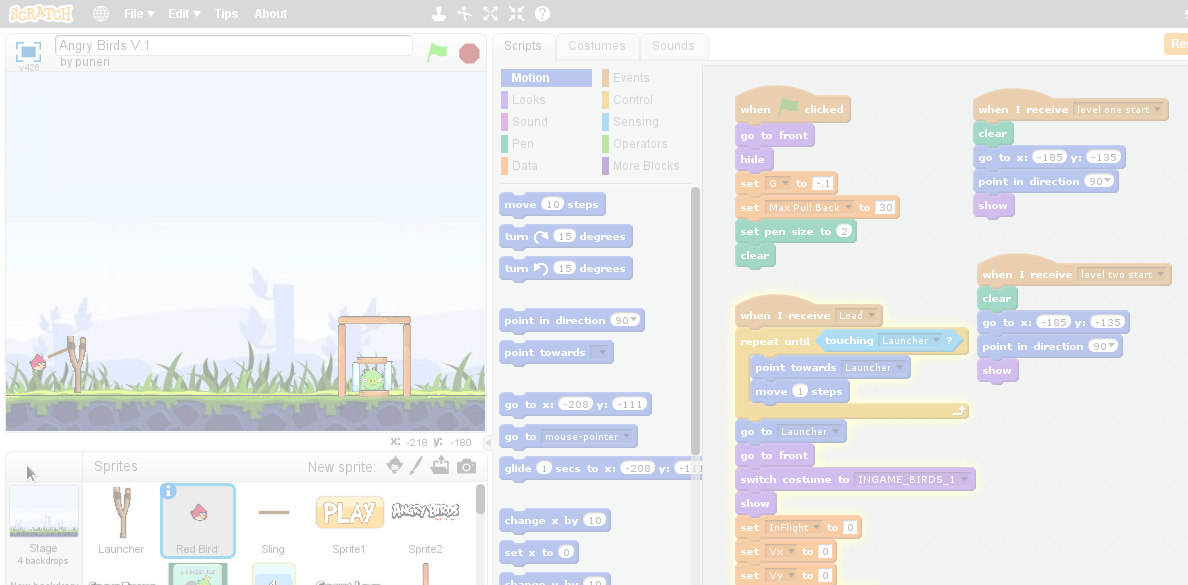
\includegraphics[width=18cm]{figs/AngryBirds2.png}}
\begin{frame}
\frametitle{Scratch}

\begin{columns}[T]
  \begin{column}{1\textwidth}
     \begin{block}{Visual programming language based on blocks}
       \begin{itemize}
         \item Designed for young learners 
         \item Massively used worldwide: 12 million users, 15 million projects
	 \item Website to share, study and remix projects, post comments or work in teams
	 \item Social aspects of sw development of FLOSS movements
       \end{itemize}
    \end{block}
  \end{column}
\end{columns}
\vspace{\baselineskip}
\hfill{\Tiny See \href{https://scratch.mit.edu/statistics/}{https://scratch.mit.edu/statistics/}}

\end{frame}
\usebackgroundtemplate{}
%--------------------------------------------------------
\usebackgroundtemplate{
\includegraphics[width=14cm]{figs/goals.jpg}}
%https://rebel-performance.com/wp-content/uploads/2014/10/goals.jpg

\begin{frame}
\frametitle{Research question}
\center{ \Large  {\bf RQ: How 'social' is the Scratch community in terms of number of comments, friends, favorites and galleries?}\\}
\vspace{\baselineskip}
\vspace{\baselineskip}
\hfill{\Tiny Background picture: rebel-performance.com}
\end{frame}

\usebackgroundtemplate{}
%--------------------------------------------------------
%--------------------------------------------------------

\begin{frame}
\frametitle{Dataset}
\begin{columns}[T]
    \begin{column}{0.5\textwidth} 
     \begin{block}{Scratch Research Data}
       \begin{itemize}
         \item Data from the Scratch online community website
         \item First five years of data, roughly 2007-2012
	 \item Core datasets, Text and Code datasets and Project Analytics datasets
       \end{itemize}
     \end{block}
    \end{column}
    \begin{column}{0.5\textwidth}
     \begin{block}{Core Dataset}
       \begin{itemize}
        \item 1,056,951 users
        \item 1,928,699 projects
        \item 120,097 galleries
        \item 1,313,200 friends
        \item 1,041,387 favorites
        \item 7,788,414 project comments
       \end{itemize}
     \end{block}
    \end{column}
  \end{columns}
\end{frame}

\usebackgroundtemplate{}
%------------------------------------------------------------

\begin{frame}
\frametitle{Results: time in the community}
\begin{center}
	\begin{figure}[t!]
		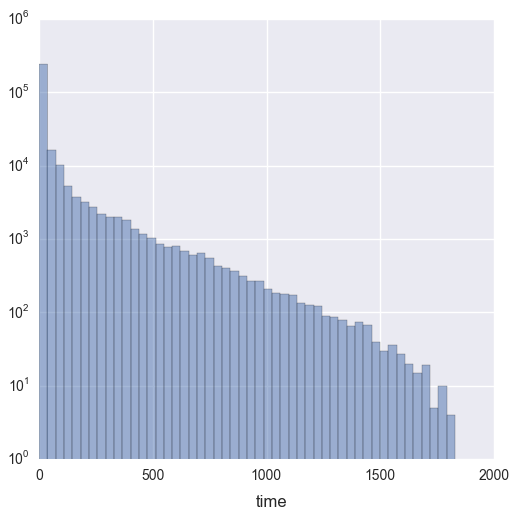
\includegraphics[width=6.5cm]{figs/time.png}    
    		\caption{Distribution of users in terms of time (days) in the community.}
	\end{figure}
\end{center}

\end{frame}

\usebackgroundtemplate{}

%%--------------------------------------------------------

%--------------------------------------------------------

\frame{
\maketitle
\begin{center}

\includegraphics[width=2cm]{format/libresoft-logo}
\hspace{0.5cm}

\includegraphics[width=5cm]{format/gsyc-urjc}
\vspace{0.5cm}

\includegraphics[width=3cm]{format/emadrid.png}
\end{center}
}

\end{document}
